\chapter{Introduction}
\label{ch:introduction}
This study is about verbs that accumulate in multi-element strings. Consider the utterance in (\ref{mehoy}) from the Austronesian language \ili{Wooi}. It consists of (at least) three verbs, each carrying the same finite marking. \figref{fig:ex1_pitch} illustrates the pro\-sod\-ic properties of the utterance. What the f$_0$ curve shows is that there is no major pitch disruption within the utterance, indicating a homogeneous intonation contour and thus (as the standard argument goes) a coherent monoclausal construction. Utterances like this one are fairly typical for many discourse genres not only in \ili{Wooi} but in many other languages around the world, and they are hard to interpret.

\begin{figure}
\begin{center}
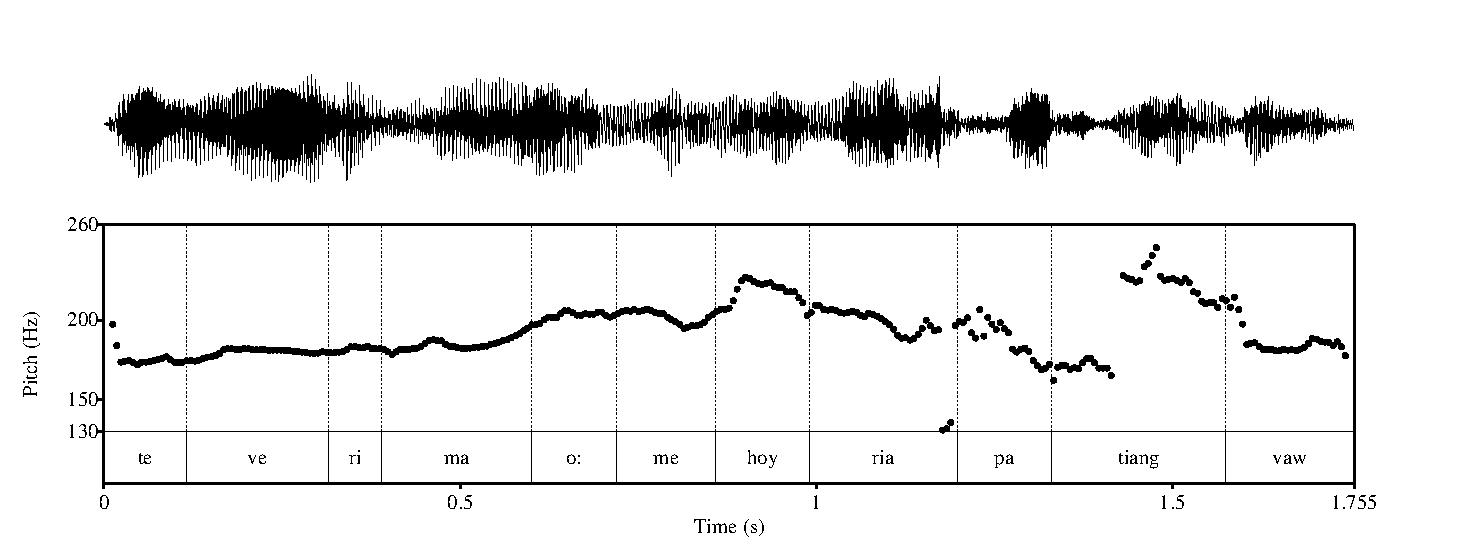
\includegraphics[width=1.0\textwidth]{figures/mehoy.eps} 
\caption{F$_0$ contour of example (\ref{mehoy})}\label{fig:ex1_pitch}
\end{center}
\end{figure}

\ea \label{mehoy}
\langinfo{Wooi}{Austronesian, SHWNG}{MOB\_1\_EW 082}\\
\glll teveri ma o: mehoy riapa tiang vaw\\
$<$i$>$taveri ma o: $<$i$>$mahoy $<$i$>$rapa tiang vaw\\
$<$3\textsc{sg}$>$return come \textsc{int} $<$3\textsc{sg}$>$sit $<$3\textsc{sg}$>$roast fish \textsc{det}:\textsc{pl}\\
\glt ‘He came back (and) sat (and) roasted the fish.’
\z

The challenge to traditional linguistic analysis is that such verb strings in many cases bear no clear signs of any grammatical relationship between the participating verbs. In the example, the verbs all appear to be of equal syntactic rank as no inflectional differences can be found.\footnote{I disregard \textit{ma} here for the moment, as there are particular problems associated with its analysis. It is one of three directional elements that occur in postverbal position, adding path semantics to motion event construals. For historical and paradigmatic reasons, I analyse \textit{ma} in \ili{Wooi} as a verb, even though it has lost its ability to inflect for subject indexing.} Thus, at first inspection they may be labelled \textit{underspecified verb sequences} as they appear to be different from the better known clause-linking types traditionally divided into coordination and subordination. The existence of such verb strings poses problems for linguistic theory. If multi-verb strings in one group of languages are mapped on units (for instance by means of translational equivalence) that in another group of languages contain only a single verb, then any traditional approach that derives syntactic units such as the clause from \emph{one} lexical head would be challenged. Or to put it another way, the one-verb-one-clause formula does apparently not qualify for all contexts in all languages \citep{foley1985clausehood}. What is more, in typical instances of clause linkage it is often clear that we are dealing with two or more individuable clauses (for instance because they receive different degrees of finite marking). Multi-verb strings, however, do not always show clear signs of clause boundaries, and so it might be suspected that, in some cases,  multi-verbal but mono-clausal structures are involved. For instance, a similar assumption is made in better known cases of secondary predicates, such as in \textit{Alice drank the coffee cold} where we would not want to claim that \textit{the coffee (is) cold} is a separate clause nested into a matrix clause \textit{Alice drank coffee}.

\section{Verb serialisation}

Some of these verb strings have stimulated a profound discussion under the heading of \emph{verb serialisation} in the last decades (important contributions include \citealt{sebba1987syntax}, \citealt{Durie1997}, \citealt{Aikhenvald2006}, \citealt{foley2010events}, \citealt{haspelmath2016serial}). Within the emerging field of serial verb analysis, some of the most basic linguistic concepts such as \emph{clause} and \emph{predicate} on the grammatical level, \emph{intonation unit} on the phonological level, and even the notoriously difficult notion of \emph{event} in the cognitive domain have since been explored in the attempt at gaining access to the hidden mechanics of these structures. The fundamental idea lurking behind the upsurge of research into serial verb constructions (henceforth SVCs) was that if no direct evidence for the status and mutual relationship of the verbs could be found, indirect evidence might be mustered by observing boundary behaviour on different planes of linguistic segmentation (grammar, prosody, gesture, eventhood etc). 

Very broadly, we may characterise two strands of reasoning that delimit the outer poles of the discussion. The first approach sets out from the assumption that SVCs are in essence little different from homologous construction types in other languages, be it on the level of syntax or on the cognitive-conceptual level. Ambiguous though those structures may look on the surface, their hidden mechanics of combination in principle follow the same rules as more familiar clause-linking constructions. Analysis, then, boils down to what \citet{givon1991serial} has called the typology of cross-language coding variability. We may dub this the \textit{nothing-new approach}. 

The second approach, on the other hand, treats verb serialisation as a phenomenon that is genuinely unique and not compatible with a multi-clausal analysis at all. For instance, \citet{foley1984functional} proposed a special nexus type in SVCs which they termed cosubordination: two constituents that are neither coordinated nor subordinated, but do show signs of mutual dependency. The view that verb serialisation is a syntactic phenomenon of its own tallies with considerations at the level of event conceptualisation and reporting. Perhaps most famous in this regard is Givón's dispute with Pawley, who claimed that a serial verb language like the Papuan language Kalam differs from English in the kinds of events that can be expressed in a single clause \citep{Pawley1987, pawley2011event}. Constraints on event packaging may be interpreted as being associated with deeper cognitive processing, and this has been taken as evidence that serialisation patterns are indicative of a marked cleavage. While some languages  allow certain events to be conceptualised with single lexical items, others require (at least some) event construals to be composed of a set of lexical items (each denoting one particular sub-event in the overall event plot). Accordingly, we may dub this second view on serial verbs the \textit{all-new approach}.

\largerpage
One of the concerns in the literature on serialisation has been the question of where to draw the boundary between SVCs and other types of (unmarked) verb combinations. While no definitive consensus has yet been reached, there is a set of construction types that appears to form the core of what is considered to constitute serialisation. Abstracting very roughly from the body of literature, constructions seem more likely to be analysed as SVCs if: (i) the verbs are dynamic rather than stative, (ii) intransitive verbs are unergative rather than unaccusative (but cp. positional verbs), (iii) the function of the ``functor verb" is comparable with a function in other languages in which a lexical item from a different part of speech is employed (``functional equivalence", for instance in case-marking, directional, aspectual SVCs etc), and (iv) the verbs encode single path trajectories rather than multiple ones as found with episodic verbs (see e.g. \citealt{pawley2011event} for discussion). 

\section{Multi-verb constructions}

Yet not all multi-verb strings have received this degree of attention. There are types of verb combinations that have been mostly excluded from consideration in the serialisation debate, a point touched upon by \citet{givon1991serial}. He pointed out that typically those constructions are omitted from discussion that in all languages are coded with more than one verb, most prominently various types of complement-taking constructions, as well as constructions in which one of the constituents receives an adverbial interpretation. To this we may add instances of modal verb constructions, periphrastic causatives, unmarked relative clauses and the like, all of which may bear a resemblance to canonical serial verb constructions. This lack of interest is somewhat remarkable inasmuch as some of these constructions \emph{prima facie} receive formal coding (or better: non-coding) in some serial verb languages that seems rather identical to canonical serialisation coding. If verb serialisation is to become more than a mere ``pre-theoretical umbrella term" as \citet{zwicky1990we} put it, analyses would need to account for such cases of coding similarity, and explain on which grounds verb serialisation \textit{proper} is indeed a different kind of verb combining than, say, a paratactic perception complement construction (e.g., the \textit{I see you come}-type). 

An alternative starting point, which I will argue for throughout this book, is to take into consideration a wider set of multi-verbal patterns, not just a subset of ``canonical" serial verbs that seem uncontroversial across the current linguistic discussion. An inclusive approach will allow the redrawing of the boundaries of verb combination types if necessary, rather than force the application of \textit{a priori} disqualification criteria, thereby risking the exclusion of related constructions from analysis altogether. This is one of the reasons why I will use the more neutral and inclusive term \textsc{multi-verb construction} (from here on abbreviated as MVC) rather than serial verb construction.\footnote{A brief disclaimer on terminology is in order here. While the term SVC has been in use for several decades (the concept ultimately dating back to \citealt{christaller1875} who used the term ``verbal phrase"), and has up to now been elaborated with a wealth of definitions, the term MVC is quite new, and thus still largely undefined. Both terms are thus hard to compare. Throughout this book, I will use the traditional term SVC for any verb string that has been defined as such in the literature on verb serialisation, except for examples that have been collected as part of my sample. All other multi-verb strings will be referred to as MVCs, that is, comprising both the data retrieved from the published sources and analysed in the subsequent chapters, as well as any other string that contains more than one verb and appears to be underspecified in the sense defined below, without necessarily showing all criteria of a SVC.} I will motivate this decision, as well as give a working definition of what I assume MVCs to be, at the end of \chapref{ch:theory}.

\section{Aim and scope of the study}

This study is intended to contribute to our understanding of MVCs by looking at two groups of languages in Eastern Indonesia (from here on EI): the Papuan languages of the Bird's Head area, Northern Halmahera as well as the Timor-Alor-Pantar group on the one hand, and the Austronesian languages spoken on Sulawesi, the islands of Nusa Tenggara, the Moluccas, and in Western Papua on the other. The sample consists of an overall 32 languages made up of 16 Austronesian languages, and 16 non-Austronesian or Papuan languages. \figref{map:overview} provides a first overview of the area as well as the languages chosen to be included in the sample.

\begin{sidewaysfigure}
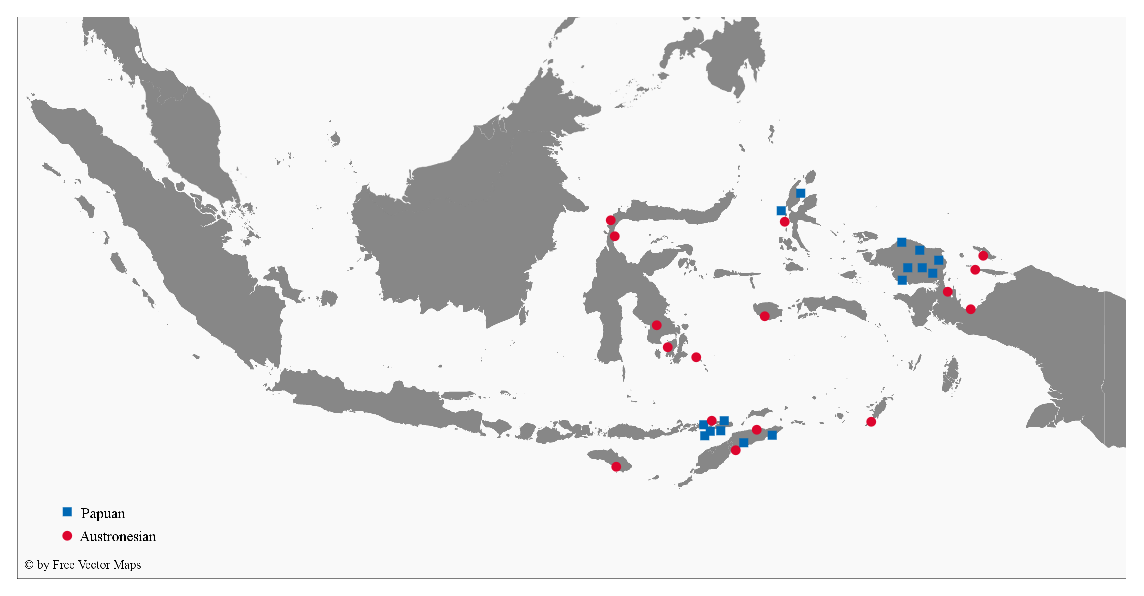
\includegraphics[width=\columnwidth]{figures/Map_overview_klein.eps}
\caption[Geographical distribution of sample languages]{Geographical distribution of the sample languages across Eastern Indonesia. Languages are grouped into Austronesian (red circles) and Papuan (blue squares).}\label{map:overview}
\end{sidewaysfigure}

The data for this work has been collected from published grammars, research papers as well as from two extensive language documentation corpora, and is introduced in §\ref{sec:data} below. In the course of this study, I will collate and discuss the grammatical (\chapref{ch:gram}) and semantic (\chapref{ch:sem}) properties of multi-verb strings in these languages. The results obtained from these sections will then in \chapref{ch:constructions} feed into a typology of MVCs. 

My analysis of MVCs from the EI region is primarily informed by the following hypotheses that I will flesh out in the chapters to come:

\begin{footnotesize}
\begin{itemize}
\item \textbf{\#Hypothesis 1:} Although the morphosyntactic make-up of MVCs in EI is remarkably similar across different construction types, these MVCs are constructed through different techniques (mentioned below in \#H2)
\item \textbf{\#Hypothesis 2:} Verbal interaction in MVC formation involves three principle techniques at the clausal level: \textsc{merging} (of features), \textsc{modification} and \textsc{staging} (alignment of spatiotemporally distinct stages)
\item \textbf{\#Hypothesis 3:} The different techniques of MVC formation are based on a layered structure of event conception, each technique being associated with a particular level of the event schema
\item \textbf{\#Hypothesis 4:} Some MVC types may be embedded into a constructional slot of another MVC resulting in \textsc{stacked MVCs}
\item \textbf{\#Hypothesis 5:} Not all EI languages use all techniques. Differences in the use of MVC patterns indicate different linguistic subareas or diffusion zones of grammatical traits. MVC use radiates out from two hotspots of MVC innovation: the Timor-Alor-Pantar and the Bird's Head region, respectively.
\end{itemize}
\end{footnotesize}

One of the goals of this work is to put together form and meaning, and explore the ways in which the languages of the sample mould the different semantic combinations into grammatical form. I will try to show that some form--function mappings are predominant in the dataset although formal encoding of MVCs in general does not immediately mirror the semantic relationship between their verbs. What is more, I will argue throughout this book that the fact that such verb strings are formally underspecified does not necessarily mean that all instances belong to the same string type nor that we invariably deal with flat concatenations of verbs. The analysis proposed in the next chapters rather rests upon the claim that some combination types in fact host embedded MVCs and are better analysed as (covert) hierarchical structures (a concept that I will metaphorically refer to as \textsc{stacked MVC}s).

A second main concern of this work is to explore the numerous treatments of serial verbs and related constructions in the languages of Eastern Indonesia. While typological research into serial verbs has been done for the Oceanic languages with considerable detail \citep{crowley2002serial, bril2004complex, bril2007nexus}, comparative analyses of Eastern Indonesian languages are still rare and largely confined to the exploratory study of \citet{vanstaden2008serial}. This book is the first attempt to explore the use of MVCs throughout all of Eastern Indonesia, including peripheral parts such as Sulawesi, by taking into account a comprehensive sample of both published data and data from extensive language documentation corpora. To my knowledge, this book represents the first research into the areal characteristics of multi-verb strings that is explicitly based on a thorough assessment of the defining properties of both SVCs and MVCs. The findings arising from this assessment will be shown to support the assumption that Eastern Indonesia constitues a Sprachbund area.

SVCs have been reported from most of the languages in Eastern Indonesia for which data are available, displaying an intriguing range of verb combinations. Some grammars allot much space to the description of SVCs, while others note their presence in passing. The heterogeneous distribution of information as well as the different theoretical underpinnings of these analyses renders such a comparative task a challenging yet also rewarding endeavour. I hope that by evaluating this wealth of constructions this work may contribute another piece to the jigsaw of finding commonalities in the diversity of verb combination patterns.

The remainder of this chapter serves as a first introduction to the phenomenon under investigation, as well as to the sample on which it is based. The next section will illustrate basic properties of underspecified verb sequences and highlight some of the analytical problems. The chapter ends with a presentation of the data sample, its various sources, and a brief discussion of the methodology used throughout the study.

\section{Underspecified verb sequences}\label{underspecified}

At the beginning of this chapter, I described serial verb structures in broad terms as underspecified verb sequences. What does \textit{underspecified} mean? \textit{Underspecified} in my sense refers to a lack of overt signals: Verbs in SVCs do not normally bear formal marks of dependency that would enable us to identify the kind of relationship holding between them. Infinitive morphology, non-finite verb forms, reduced verbal inflection, as for instance with medial verbs or converbs: all such devices are typically not found in SVCs, so that potential hierarchical relationships between the verbal constituents are not cued directly. In fact, it appears that we do not even know whether there \emph{is} a particular grammatical relationship present between the verbs, or whether the verbs are placed next to each other in loose apposition. If this turned out to be true, we might better understand the verbs as put together only on the output level of prosodic segmentation rather than on the syntactic level of constituent structure, in much the same way as, say, a phonological word may string together constituents that, from a grammatical perspective, constitute independent units. This idea is not at all implausible as natural speech data show, and I will return to this issue briefly in \chapref{ch:discussion}. 

For now, suffice it to say that underspecified means here that verbs in serial verb languages typically are not grammaticalised with regard to being capable of expressing different degrees of finiteness. This does not mean that verbs in these languages do not inflect for verbal categories such as person marking or TAM categories. They may do so, and, in fact, most languages in the EI sample inflect for one category or another. The crucial point is that verbal inflection in most of these languages is not structurally exploited in such a way as to systematically encode differences in verbal hierarchy.\footnote{While this seems to hold for most of the languages I have looked at, there are notable exceptions, where languages do provide finiteness options to mark off certain construction types. In the Papuan language \ili{Yimas}, for instance, simultaneous events have to be marked by a non-finite oblique case-marking nominalization \citep[142]{foley2008}, whereas sequential event chains may be encoded by SVCs.} At least in the EI languages, presence or absence of inflection is governed by phonological rules or membership to a certain verb class rather than by restrictions imposed by SVCs.

Let us now turn to some examples. The examples below are chosen to illustrate the most frequent formal and semantic characteristics of SVCs in the literature. They are taken from the major linguistic areas for which serialisation has been reported: West Africa, China, and also Papua (see \citealt[2]{senft2008intro}), are the areas in which early language descriptions first spotted serialised verb patterns \citep{sebba1987syntax, Matthews2006}. \citet{christaller1875}, with his account of the Twi language (\ili{Akan}), spoken in Ghana, is usually credited with being the first explicit description of serial verb constructions. The linguistic discussion of serialisation later spread to Creole languages (starting with Atlantic Creoles, later followed by Pacific and South Asian Creoles; see \citealt{nordhoff2012}), and later again to Papuan and Austronesian languages in the Pacific area, mainland Southeast Asia and South America \citep{senft2008event}. Linguistic descriptions of SVCs from these areas have all contributed greatly to our understanding of verb combination types, and some of the defining features of SVCs occur over and over again.\footnote{Note that many of these examples contain free translations that seem somewhat confusing to scholars beginning to study SVCs. In order to render the meaning of SVCs into well-formed English, conjunctions are often inserted into translations. Conjunctions (and other material) in brackets should therefore not be taken literally but understood as stylistic means to facilitate understanding. The same goes for conjunctions that are not in brackets but do not have a corresponding morpheme in the transcription tier. I have refrained from altering the free translation of examples where the author did not indicate stylistic additions so as to not violate the utterance meaning, or to hamper alternative analyses on the reader's part.}

\ea \label{Twi0001} 
West Africa\\
\ea \label{Twi01}
\langinfo{\ili{Akan} (Twi)}{Niger-Congo}{\citealt{christaller1875}, quoted in \citealt[21]{ameka2005multiverb}}\\
\gll Yε-\textbf{sɔre}-e ntέm \textbf{kɔ}-ɔ  fie.\\
\textsc{1}\textsc{pl}-rise-\textsc{pst} quickly go-\textsc{pst} home\\
\glt ‘We arose [got up, F. K. Ameka] quickly (and) went home.’
\ex \label{Ewe01}
\langinfo{\ili{Ewe}}{Niger-Congo}{\citealt[135]{ameka2006ewe}}\\
\gll e-\textbf{kó} fiá kó \textbf{dzá} ati-a \\
\textsc{3}\textsc{sg}-raise axe take hack stick-\textsc{def}\\
\glt ‘He used an axe and hacked the wood.’
\z
\z

\ea
Sinitic languages\\
\ea \label{Man01}
\langinfo{\ili{Mandarin}}{Sino-Tibetan}{\citealt[96]{LiThompson1973}}\\
\gll Zhāng-sān \textbf{chuān-shang} yīfu \textbf{tiào} zai dì-shang\\
Zhang-san put-on clothes jump on floor\\
\glt ‘Zhang-san put on his clothes and then jumped on the floor.’
\ex \label{Can01}
\langinfo{\ili{Cantonese}}{Sino-Tibetan}{\citealt{omelia1966first}, quoted in \citealt[69]{Matthews2006}}\\
\gll keoi$^5$ \textbf{jap$^6$} \textbf{heoi$^3$} \textbf{co$^5$}\\
\textsc{3}\textsc{sg} enter come sit\\
\glt ‘He went in and sat down.’
\ex \label{Can02}
\langinfo{\ili{Cantonese}}{Sino-Tibetan}{\citealt[75]{Matthews2006}}\\
\gll keoi$^2$ \textbf{haam$^3$}-\textbf{sap$^1$}-zo$^2$ go zam$^2$tau$^4$\\
\textsc{clf} cry-wet-\textsc{prfv} \textsc{clf} pillow\\
\glt ‘She's made her pillow wet by crying.’
\z
\z

\ea
Creole languages\\
\ea \label{Sra01}
\langinfo{\ili{Sranan}}{English based Creole, Atlantic}{\citealt[50]{sebba1987syntax}}\\
\gll Kownu \textbf{seni} wan boskopu \textbf{gi} tigri\\
King send a message give tiger\\
\glt ‘King sent Tiger a message/a message to Tiger.’
\ex \label{Sra02}
\langinfo{\ili{Sranan}}{English based Creole, Atlantic}{\citealt[40]{sebba1987syntax}}\\
\gll \textbf{lon} \textbf{go} \textbf{teki} a buku \textbf{tyari} \textbf{go} \textbf{gi} a leriman\\
run go take the book carry go give the teacher\\
\glt ‘Run and fetch the book and take it to the teacher.’
\z
\z

\ea
Papuan region\\
\ea \label{Ala01}
\langinfo{\ili{Alamblak}}{Papuan, Sepik}{\citealt[20]{bruce1988}}\\
\gll wa-ha-\textbf{muh}-\textbf{hɨta}-tañ-ñ-m-ko\\
\textsc{imp}-\textsc{caus}-climb-put-\textsc{compl}-\textsc{2}\textsc{sg}-\textsc{3}\textsc{pl}-up\\
\glt ‘Lift them up (and) leave them up here.’
\ex \label{Ala02}
\langinfo{\ili{Alamblak}}{Papuan, Sepik}{\citealt[20]{bruce1988}}\\
\gll \textbf{tat}-\textbf{noh}-më-an-r\\
hit-die-\textsc{rpst}-\textsc{1}\textsc{sg}-\textsc{3}\textsc{sg}.\textsc{m}\\
\glt ‘I killed him by hitting (him).’
\ex \label{Yim01}
\langinfo{\ili{Yimas}}{Papuan, Ramu-Lower Sepik}{\citealt[80]{foley2010events}}\\
\gll arm-n kay i-ka-\textbf{ak}-mpi-\textbf{wul}\\
water-\textsc{obl} canoe.\textsc{viiisg} \textsc{viiisg}.\textsc{obj}-\textsc{1}\textsc{sg}.\textsc{act}-push-\textsc{seq}-put.in\\
\glt ‘I pushed the canoe down into the water.’
\z
\z

\ea \label{Paa0001} 
Oceanic region\\
\ea \label{Paa01}
\langinfo{Paamese}{Austronesian, Oceanic}{\citealt[55]{crowley2002serial}}\\
\glll inau \textbf{nuas} vuas \textbf{he:mat} \\
inau ni-uasi vuasi hee-mate\\
\textsc{1}\textsc{sg} \textsc{1}\textsc{sg}.\textsc{dist}.\textsc{fut}-hit pig \textsc{3}\textsc{sg}.\textsc{dist}.\textsc{fut}-die\\
\glt ‘I will hit the pig to death.’
\ex \label{Paa02}
\langinfo{Paamese}{Austronesian, Oceanic}{\citealt[60]{crowley2002serial}}\\
\glll i:r \textbf{reheso:n} vakili \textbf{he:ha}\\
iire rehe-sooni vakilii hee-haa\\
\textsc{1}\textsc{pl}.\textsc{in} \textsc{1}\textsc{pl}.\textsc{in}.\textsc{dist}.\textsc{fut}-throw canoe \textsc{3}\textsc{sg}.\textsc{dist}.\textsc{fut}-go\\
\glt ‘We will throw the canoe away.’
\z
\z

If we just compare the visible surface features of these constructions, we see both variation between languages, and shared feature values. At the level of constituent order, the serial verbs may either form a coherent group, as in (\ref{Can01}), (\ref{Can02}), (\ref{Sra01}), (\ref{Ala01}), (\ref{Ala02}), (\ref{Yim01}), or their sequence may be broken up by other constituents, as in (\ref{Twi01}), (\ref{Ewe01}), (\ref{Man01}), (\ref{Sra01}), (\ref{Sra02}), (\ref{Paa01}), (\ref{Paa02}). If the first verb is transitive and the direct object is overtly expressed, the argument may either stand right after the verb (cp. (\ref{Ewe01}), (\ref{Man01}), (\ref{Sra01}), (\ref{Sra02}), (\ref{Paa01}), (\ref{Paa02})), or the verbs may form a tight unit with the object in preverbal position or after the last verb in the series, as in (\ref{Can02}), (\ref{Yim01}). Yet even if the first verb is intransitive, the construction may still permit the insertion of a modifier (as the adverb \textit{ntέm} in (\ref{Twi01}) from \ili{Akan} shows). 

Another criterion that shows variation is word boundaries: a sequence of serial verbs may either form one phonological word, or each verb may constitute an independent word. Many Papuan languages combine verbal roots at the morphological level, but example (\ref{Can02}) shows that the phenomenon may also occur in other areas. If the verbs come to stand within one phonological word, it may be difficult to distinguish serialisation (which started its linguistic career essentially as a syntactic phenomenon) from verbal compounds (see e.g. \citealt{vanstaden2008serial} for discussion). Some writers like \citet{devries2004} have argued that stress assigment is an indicator of whether a multi-verbal root structure constitutes a compound (one stress peak) or a phrasal construction (stress peak on each root). \citet{vanstaden2008serial} explicitly exclude root combinations with only one primary accent from the group of serial verb constructions in spite of striking semantic similarities. \ili{Inanwatan}, for instance, has no serial verbs, according to their analysis, but only verbal compounds. In this study, I will take a more liberal stance on these structures and will subsume both under the heading of \textit{multi-verb construction}, for the following reasons. First, stress assignment in multi-root structures is not always clear from the data sources. Second, it has been claimed that serial verb structures may evolve into compounds at some point (see \citealt[27]{vanstaden2008serial}), and so we might expect \isi{serialisation} structures and \isi{compound}s to be conceptually similar. And third, some compounds fit into semantic types that are otherwise observed in serial verbs, so that it seems more interesting to include such cases at this point. 

The main weakness of the stress test is the presupposition that the language in question does have a word-level prosodic system that enables the distinction between verbal compounds and (word-level) serialisation. In general, the presence or absence of features used to confirm the existence of SVCs indeed poses a well-known problem. Not all languages show all features. This is pointed out by \citet[22]{vanstaden2008serial}: 

\begin{quote}What often obscures the discussion on serial verb constructions is [...] that criteria that can be applied in one language to distinguish, for instance, SVCs from subordination or compounding, simply may not be applicable for other languages.\end{quote}

For instance, if we compare the inflection marks on the verbs in (\ref{Twi0001})--(\ref{Paa0001}) above, we are not able to define a clear \textit{tertium comparationis}: some of the languages show person marking on the verbs (\ili{Ewe}, \ili{Yimas}), others (may) mark TAM values (\ili{Mandarin}, \ili{Cantonese}), and still others have both (\ili{Akan}, \ili{Alamblak}, \ili{Paamese}) or no inflectional marking at all (\ili{Sranan}). Presence or absence of verbal morphology is often used to infer a hierarchical status of the constituent, and inflected verbs may be analysed as being head of a specific construction. A difference in verbal inflection between the verbs in a SVC could therefore be taken as evidence that the uninflected verb is of a lower rank than the inflected (matrix) verb. The \ili{Akan} and \ili{Ewe} examples above could be interpreted in such a way. 

A related factor that might also indicate differences in verbal rank is the overt expressability of arguments in a SVC. In the \ili{Cantonese} and \ili{Paamese} examples, we see that the subject argument is only expressed once as a pronoun before the first verb. The second verb does not trigger the use of a subject pronoun. While pronoun assignment may in general be governed by more general pragmatic factors in pro-drop languages, the \ili{Paamese} data show that there are hidden restrictions at work in particular constructions. \citet{crowley2002serial} observes that in examples such as (\ref{Paa01}) overt expression of the second subject (which is co-referential with the object of the first verb) is not licit. If an independent pronoun is inserted into the preverbal subject slot of the second verb, the construction apparently changes with regard to two properties: (i) the interpretation of the event becomes sequential (`hit the pig and it will die' instead of `hit the pig to death'), and (ii) it becomes possible to insert the coordinator \textit{kaa} `and' between the verbal constituents without any clear change in meaning. This is evidence that in \ili{Paamese} switch subject constructions, the second verb has a deranked status and does not show full independence with regard to subject assignment.

Summing up this brief analysis of the examples, we have seen that there are several parameters with different possible values in SVC formation, for instance verbal inflection patterns, constituent placement and argument realisation. The same amount of variation is found in the semantics of verb combinations. \citet{givon1991serial} classified SVCs into five distinct functional types:

\begin{footnotesize}
\begin{itemize}
\item \textbf{Case-role marking}: A functor verb is grammaticalized into a verbal case marker of different sorts of core or oblique arguments, for instance patient, benefactive, instrumental, or locative
\item \textbf{Co-lexicalization}: Two verbs are co-lexicalized and form a more complex verbal concept
\item \textbf{Deictic-directional marking}: Deictic directional verbs like `come' or `go' lend their deictic meaning to other verbs of motion or transport creating complex deictic expressions of motion in space
\item \textbf{Tense-aspect marking}: A functor verb is grammaticalized into a marker of aspectual or modal function
\item \textbf{Evidentiality and epistemic marking}: a functor verb has acquired a reading of evidentiality
\end{itemize}
\end{footnotesize}

aOf these broad functions, case-role marking, co-lexicalisation, deictic-direc\-tion\-al marking, and, to a lesser extent, tense-aspect marking can also be found in the languages of Eastern Indonesia. Example (\ref{Ewe01}) is a good instance of the case-role marking type: the argument \textit{fiá} `axe' is introduced as a theme argument by the first verb \textit{e-\textbf{kó}} `raise/take'. At the same time, one can argue that, within the particular context of the construction, it also serves as the instrument to the action of hacking, and thus \textit{e-\textbf{kó}} might be analysed as a grammaticalised verbal instrument marker. The co-lexicalisation scenario can possibly be observed in the second \ili{Cantonese} example (\ref{Can02}).

Yet with all this variation in place, SVCs do show signs of similar overall construal. There are no morphological cues to differences in verbal hierarchy (other than differences in verbal inflection). There are no connectors, conjunctions, complementisers or other formatives between the verbs (\ili{Yimas} \textit{-mpi-} provides an exception here). TAM values (e.g. the past marker \textit{-e/-ɔ} in (\ref{Twi01}) or the remote past marker \textit{-më} in (\ref{Ala02})) or markers of illocutionary force (as imperative \textit{wa-} in (\ref{Ala01})) are canonically interpreted as having scope over the entire construction. All verbs share at least one of their arguments with each other. And for many languages, SVCs have been reported to occur under a coherent intonation contour, suggesting that on the prosodic level the verbs are grouped into one homogeneous unit.

The features presented in this brief preview will be taken up again in the following chapters, and will be critically examined as to whether or not they may be applied to the EI sample. In \chapref{ch:theory}, an analysis of the defining properties of serial verb constructions is laid out. We shall see that not all features are equally useful, or else they cannot be applied without resorting to further properties that, from language to language, may be quite different. While I will eventually single out three morphosyntactic properties that are put to the test in \chapref{ch:gram}, the results  show, I will argue, that looking at morphosyntactic properties alone will not give rise to any meaningful analysis. In \chapref{ch:sem}, the analysis will therefore shift to a semantic approach, identifying four underlying techniques of MVC formation at different conceptual levels. It is these semantic techniques that will then in \chapref{ch:constructions} feed into a typology of MVCs. Quite unlike Givón's functional typology of SVCs from above, we will arrive at four constructional families that each accomodate a set of constructions that is in use across most of EI.

In the next section, I turn to my area of research and briefly introduce the sample on which this study is based.

\section{Data sample and methodology}\label{sec:data}

As already mentioned, this study was primarily designed as a literature survey in order to gather data on SVCs in the area of Eastern Indonesia that would otherwise remain ``tucked away" in grammars and research papers. By collating data from different EI languages, both Austronesian and Papuan, I explore the wealth of construction types, their distribution and distinct properties in this area. To this end, I identified 30 languages for which sufficient published data were available. This set of published data was further complemented with another two languages for which extensive language documentation corpora were available: \ili{Waima'a} and \ili{Wooi}. Both languages had been investigated in DoBeS language documentation projects (I was part of the \textit{Documenting Wooi} project), and I had sufficient working experience with them. 

The languages for the literature survey were chosen to meet the following conditions:

\begin{footnotesize}
\begin{itemize}
\item Enough material for at least 25 data points from a range of different constructions\footnote{Except, of course, for EI languages that only make very limited use of serial verbs, or do not use them in the first place. All languages reviewed for the data set turned out to use at least some MVCs, so that all languages can be said to meet this condition. Only Austronesian \ili{Selaru}, spoken in the southern Moluccas, appears to have developed a small set of linking elements that are extensively used throughout what otherwise looks just like ordinary MVCs.}
\item A grammatical description dealing with SVCs and their language-specific properties
\item Sufficient geographical and genetic variation within the data set to model all subareas and taxa
\item Recent publications
\end{itemize}
\end{footnotesize}

\tabref{table:sample} below gives an overview of the languages that were included in the sample. The first goal, at least 25 (varied) data points, was easy to achieve as most book-length publications included numerous varied examples of SVCs. The normal form for grammars to deal with the topic is to devote an exclusive chapter or section to the discussion of serial verbs. Therefore, the second requirement was also met by almost all data sources. Very few publications deviated from this pattern, but were included nonetheless: The grammars on \ili{Abun} \citep{berry1999} and \ili{Makalero} \citep{huber2011} do not directly discuss serial verbs, nor does the sketch grammar on \ili{Dusner} \citep{dalrymple2012}. They were included as they displayed many SVCs among their examples in other sections. The \ili{Mor} data paper \citep{kamholz2009} is another exception, since it does not contain any grammatical description but only an interlinearised text and a dictionary. As an outlier to both the Bird's Head area as well as to the South Halmahera-West New Guinea taxon, I decided to include \ili{Mor} nonetheless, treating it as if the data were taken from a language documentation corpus like the ones for \ili{Waima'a} and \ili{Wooi}.

The third goal was to include as many sub-branches of the language families as possible, and to attain a geographical distribution of the sample languages that would cover different subareas in EI. To this end, I tentatively assumed four subareas for which rather homogeneous MVC features might be expected: Sulawesi and Western (Bird's Head) Papua were chosen as subareas because of their geographical coherence and their linguistic profile, with the former showing most western Austronesian features, and the latter displaying the central diffusion zone of (West) Papuan features into adjacent Austronesian languages. Two further subareas have been defined in central Wallacea: Nusa Tenggara comprises the lesser Sunda Islands from Flores in the west up to the Timor achipelago including Alor and Pantar. Finally, Maluku comprises the area from the Aru Islands in the south, across Banda and Seram and up to the Halmahera archipelago in the north. A subdivision of Eastern Indonesia into these four subareas is also supported by findings from biogeographical dispersal barriers through the region. The borders of the subareas match with the biological demarcation lines briefly outlined in §\ref{sec:area_intro} (cf. \figref{map:wallacea} for an overview).\footnote{The only exception to this is the border between the subareas of Nusa Tenggara and Maluku. Following Zollinger's Line would require the inclusion of \ili{Selaru} into the Nusa Tenggara group (see \figref{map:wallacea}). As Selaru appears to share more characteristics with \ili{Buru} than with Austronesian languages spoken on Timor, I rather placed \ili{Selaru} with the languages of the Maluku group.} \figref{map:subareas} illustrates the four subareas and their associated languages. 

\begin{sidewaysfigure}
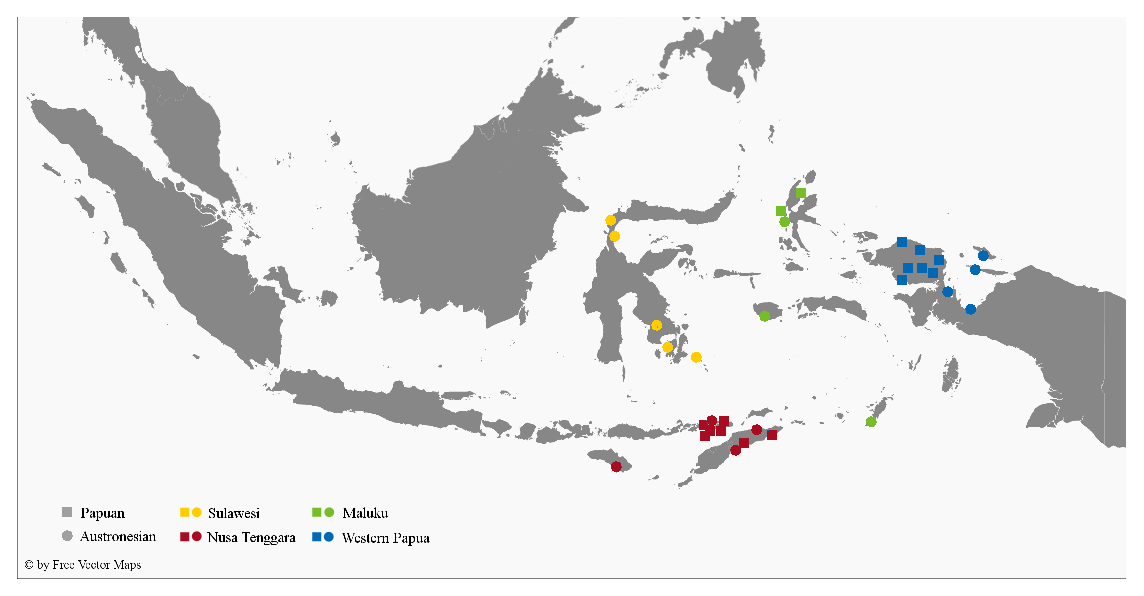
\includegraphics[width=\columnwidth]{figures/Map_overview_klein_subareas.eps}
\caption[Geographical distribution of the sample languages across subareas]{Geographical distribution of the sample languages across the four subareas Sulawesi, Nusa Tenggara, Maluku, and Western Papua. Languages included in the sample are given in coloured squares (Papuan) and circles (Austronesian).}\label{map:subareas}
\end{sidewaysfigure}

As can be seen from \tabref{table:sample}, the number of sample languages in the different subareas is not as balanced as I hoped. For both Western Papua and Nusa Tenggara there were a lot of recent grammars available, especially for the Papuan languages of the Bird's Head and the Timor-Alor-Pantar area, both of which have attracted much attention throughout the last decades. Sulawesi is also covered by some excellent grammars though the area that is probably most interesting to a survey on serial verbs is the transition area in Southeast Sulawesi, for which only \ili{Muna} \citep{vandenberg1989} and \ili{Tukang Besi} \citep{donohue1999} have received fully fledged grammatical descriptions so far. Another lesser studied area in terms of published grammars seems to be the Maluku region. As a result, both the Maluku area and Sulawesi remain underrepresented in my sample, while the TAP area and the Bird's Head contributed most languages (and data points).

\begin{table}[p]
\begin{scriptsize}
\begin{tabular}{>{\footnotesize}l >{\footnotesize}l >{\scriptsize}p{3.2cm} >{\scriptsize}l r r r}
\lsptoprule
\multicolumn{1}{l}{Group} & 
\multicolumn{1}{l}{Language } & 
\multicolumn{1}{l}{Source} & 
\multicolumn{1}{l}{Type} & 
\multicolumn{3}{c}{Data points}\tabularnewline\cmidrule(lr){5-7}
\multicolumn{1}{l}{} & 
\multicolumn{1}{l}{} & 
\multicolumn{1}{l}{} & 
\multicolumn{1}{l}{} &
\multicolumn{1}{c}{ex} & 
\multicolumn{1}{c}{grm} & 
\multicolumn{1}{c}{txt}\tabularnewline
\midrule
\multirow{5}{*}{\rotatebox[origin=c]{90}{Sulawesi}}
&\ili{Muna}&\citealt{vandenberg1989}&grammar&$  0$&$ 39$&$ 11$\tabularnewline
&\ili{Pendau}&\citealt{Quick2007}&grammar&$  0$&$ 51$&$  0$\tabularnewline
&\ili{Tajio}&\citealt{mayani2013grammar}&grammar&$  0$&$ 27$&$  5$\tabularnewline
&\ili{Tolaki}&\citealt{mead2008verb}&article&$  0$&$ 65$&$  0$\tabularnewline
&\ili{Tukang Besi}&\citealt{donohue1999}&grammar&$  0$&$ 48$&$ 22$\tabularnewline
\midrule
\multirow{11}{*}{\rotatebox[origin=c]{90}{Nusa Tenggara}}
&\ili{Abui}&\citealt{kratochvil2007grammar}&grammar&$  0$&$109$&$  0$\tabularnewline
&\ili{Alorese}&\citealt{klamer2011alorese}&sketch grammar&$ 21$&$ 11$&$ 15$\tabularnewline
&\ili{Bunaq}&\citealt{schapper2009bunaq}&grammar&$  0$&$ 87$&$  0$\tabularnewline
&\ili{Kaera}&\citealt{klamer2014kaera}&sketch grammar&$  8$&$ 16$&$  0$\tabularnewline
&\ili{Kambera}&\citealt{klamer1998grammar}&grammar&$ 6$&$ 32$&$  6$\tabularnewline
&\ili{Klon}&\citealt{baird2008grammar}&grammar&$ 43$&$ 57$&$  0$\tabularnewline
&\ili{Makalero}&\citealt{huber2011}&grammar&$76$&$  0$&$  0$\tabularnewline
&\ili{Teiwa}&\citealt{klamer2010grammar}&grammar&$  2$&$ 74$&$  9$\tabularnewline
&\ili{Tetun Fehan}&\citealt{vanklinken1999grammar}&grammar&$  7$&$ 66$&$  0$\tabularnewline
&\ili{Waima'a}&\citealt{belo2002-2006}&corpus&$  0$&$  0$&$176$\tabularnewline
&\ili{Western Pantar}&\citealt{holton2014western}&sketch grammar&$  4$&$ 34$&$  0$\tabularnewline
\midrule
\multirow{5}{*}{\rotatebox[origin=c]{90}{Maluku}}
&\ili{Buru}&\citealt{grimes1991buru}&grammar&$ 10$&$ 55$&$ 3$\tabularnewline
&\ili{Selaru}&\citealt{coward2005}&grammar&$ 13$&$  0$&$ 12$\tabularnewline
&\ili{Taba}&\citealt{bowden2001taba}&grammar&$  0$&$ 32$&$ 12$\tabularnewline
&\ili{Tidore}&\citealt{vanstaden2000tidore}&grammar&$  54$&$ 12$&$ 26$\tabularnewline
&\ili{Tobelo}&\citealt{holton2003tobelo}&sketch grammar&$ 31$&$ 7$&$ 6$\tabularnewline
\midrule
\multirow{11}{*}{\rotatebox[origin=c]{90}{Western Papua}}
&\ili{Abun}&\citealt{berry1999}&grammar&$ 33$&$  0$&$  0$\tabularnewline
&\ili{Biak}&\citealt{vanheuvel2006}; \citealt{mofu2008biak}&grammar&$ 33$&$ 17$&$ 17$\tabularnewline
&\ili{Dusner}&\citealt{dalrymple2012}&sketch grammar&$ 33$&$  0$&$ 16$\tabularnewline
&\ili{Hatam}&\citealt{reesink1999grammar}&grammar&$  0$&$ 49$&$  0$\tabularnewline
&\ili{Inanwatan}&\citealt{devries2004}&grammar&$ 14$&$  4$&$ 10$\tabularnewline
&\ili{Maybrat}&\citealt{dol2007grammar}&grammar&$ 28$&$ 50$&$  0$\tabularnewline
&\ili{Mor}&\citealt{kamholz2009}&paper (text \& dict)&$  0$&$  0$&$ 71$\tabularnewline
&\ili{Moskona}&\citealt{gravelle2010grammar}&grammar&$  0$&$ 79$&$  0$\tabularnewline
&\ili{Mpur}&\citealt{ode2002sketch}&sketch grammar&$ 11$&$  7$&$ 44$\tabularnewline
&\ili{Sougb}&\citealt{reesink2002grammar}&sketch grammar&$ 20$&$  7$&$  13$\tabularnewline
&\ili{Wooi}&\citealt{kirihio2009dobes}&corpus&$  0$&$  0$&$190$\tabularnewline
\midrule
Subtotal& & & &$ 447$&$ 1035$&$ 664$\tabularnewline
Total&$ 32$& & & & & $ 2146$\tabularnewline
\lspbottomrule
\end{tabular}
\caption[Overview of the EI dataset]{Overview of the languages and the different types of data used. Further explanation in the prose.}
\label{table:sample}
\end{scriptsize}
\end{table}

If data points of MVCs were only collated from the chapters and sections specifically devoted to them, one could wonder whether the sample was indeed representative for the language, or whether the author was in some sense biased. Such a bias could, for instance, arise because a certain class of constructions attracted specific attention in the literature at that time, or because the author was intrigued by some unusual property. I tried to account for this potential bias by also checking other chapters/sections of the respective publication and noting down MVCs from examples meant to illustrate quite different things. Occurrences of MVCs in unrelated examples proved that MVCs in those language were not uncommon at all. Accordingly, I differentiated between data points from SVC discussions (\textit{grm} in \tabref{table:sample}) and data points from unrelated chapters/sections (which I counted as \textit{ex}). In cases where I felt that I did not have enough data points at hand, or where the construction types seemed not to reflect the total breadth of MVCs in a language, I also collected further examples from appended interlinearised texts (where available). These data points were glossed as \textit{txt}. The two language documentation corpora, for \ili{Waima'a} and \ili{Wooi}, served as further data sources for the two subareas Nusa Tenggara and Western Papua. All in all, I gathered 2146 examples of MVCs from 32 languages in EI.

In the next chapter I turn to the Eastern Indonesian region. I will show that a linguistic definition of EI can be based on typological and genetic grounds, and that this definition aligns well with both biological and geographical patterns. I will first introduce the region as a linguistic area, followed by an introduction to the languages that make up the sample upon which this work is based. As a basic understanding of the EI languages as well as of the literature on serialisation is required in order to interpret the sample, I defer a more thorough discussion of how I collated the EI data to the end of \chapref{ch:theory}.
